\begin{chapter}{Restlessness}
    \label{chap:restlessness}

    \begin{figure}
        \centering
        
\includegraphics[width=5cm]{source/images/restlessness_logo.png}
        \caption{The Restlessness logo}
    \end{figure}

    % Framework vs Library
    % Frameworks and libraries are both code written by someone else that helps you
    % perform some common tasks in a less verbose way.
    % A framework inverts the control of the program. It tells the developer what
    % they need. A library doesn’t. The programmer calls the library where and when
    % they need it.

    The Open Source framework named Restlessness was born with the goal of improving
    the developer experience of the Serverless framework, by addressing its encountered
    problems (\ref{subsec:sls_disadvantage}).
    The framework is composed by a Command Line Interface and a frontend application
    with an associated web server running locally.
    In particular the main functionalities that the framework aims to provide are:
    \begin{itemize}
        \item Creation of a new project, through the CLI, based on the typescript
            language, with a standard structure and based on the functionalities
            already offered by the Serverless framework.
        \item A local Web Interface that allows creating and managing project resources,
            functions, with their associated events, and models.
        \item The creation of a standard unit testing structure for each function,
            and based on the \href{https://www.npmjs.com/package/jest}{jest} library.
        \item A standard validation structure for function's input, based on the
            \href{https://www.npmjs.com/package/yup}{yup} library.
        \item Deploy of multiple services with a single CLI command, to deal with
            the resource threshold limitation of Aws, and to manage and structure
            the created project following a micro services approach.
        \item Possibility to extends the framework functionalities.
    \end{itemize}
    By addressing those points the framework aims to give developers the tools to
    focus on writing business code rather than spend time on boundary problems,
    that are important, but there may be the risk of solving the same problems
    multiple times (reinventing the wheel), which may be avoided.

    Restlessness is composed by different modular components, listed here:
    \begin{itemize}
        \item Restlessness core: core package of the framework, it contains all the
            classes and functions that provides the framework functionalities. It is
            available as \mbox{\textit{@restlessness/core}} package on npm.
        \item Command Line Interface: together with the Web Interface, this is the
            main component with which users interact the most. It depends on the
            core package to provide its functionalities, and it is available as
            the \mbox{\textit{@restlessness/cli}} package on npm.
        \item Restlessness backend: api service running locally, created with the
            Restlessness framework itself. It is used by the Web Interface to
            provides its functionalities.
        \item Restlessness frontend: Web Interface with which it is possible to
            create resources and manage the project. It is part of the CLI.
    \end{itemize}
    \begin{figure}
        \centering
        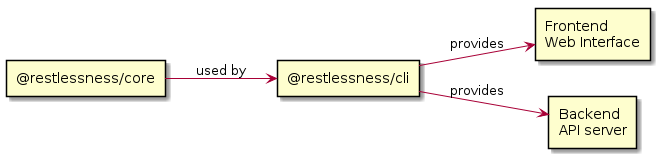
\includegraphics[width=\linewidth]{source/diagrams/rln_components.png}
        \caption{Restlessness main components}
    \end{figure}

    \section{Core}
    The core package contains the core logic components of the framework, which
    are: creation and management of resources, code generation based on templates,
    and handling of defined functions execution.
    The main resources that can be created are:
    \begin{itemize}
        \item Endpoints: endpoints are Serverless functions, triggered by and http
            event, as shown on \ref{subsec:lambda_invocation}.
        \item Schedules: schedules are Serverless functions, triggered by a
            programmed event, such as a cron job or a rate event, which is an
            event that is fired up periodically, based on the time interval provided.
        \item Authorizers: extension packages, providing Authorizer functions, as
            defined on \ref{subsec:lambda_invocation}.
        \item Daos: extensions packages, providing Data Access Object functionalities.
        \item Models: classes modeling resources, such as a User saved into a database.
            They can be associated to a Dao package, which provides its own model
            creation template.
        \item Envs: environment files, used to store information in key/value format,
            from both the user and the framework with its extensions.
        \item Services: Serverless services (i.e. \textit{serverless.json}).
    \end{itemize}

    The framework allows the creation of those resources and needs to save that
    information to be able to remember the project state, so it creates a series
    of configuration files, one for each resource type, and store them under the
    \textit{config/} directory, in JSON format \cite{json_iso}.
    It has been decided to format all configuration files across the project using JSON,
    preferring it to alternatives, such as Yaml, to simplify their handling and modification
    by the framework, given that Typescript handle JSON files and objects natively.
    Given the similar structure between those files, a single abstract class models
    it, while subclasses implement specific behaviors, following the structure
    shown in figure \ref{fig:rln_json_config_file}. Each file entry has a type
    extending the interface \mbox{\textit{JsonConfigEntry}}, which contains an entry
    identifier. This structure is achieved using the Typescript feature called
    \textit{Generic Types}
    \cite{ts_generics}.

    \begin{figure}
        \centering
        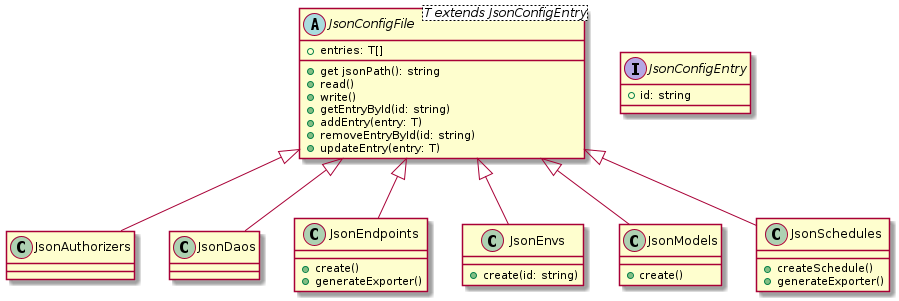
\includegraphics[width=\linewidth]{source/diagrams/rln_config_files.png}
        \caption{Configuration file classes structure}
        \label{fig:rln_json_config_file}.
    \end{figure}

    Resources created through Restlessness need to find a correspondence on the
    Serverless configuration file (\textit{serverless.yml} or \textit{serverless.json}).
    Moreover it has been decided to let the framework manages more than one service at
    a time associated to the same application or project, due to a platform limitation,
    as described on \ref{subsec:application_micro_services}.
    The structure adopted by the framework is to save the configuration file of
    each service under the \textit{serverless-services} folder, and to provide by
    default two services, as shown on figure \ref{fig:sls_services_dir}.
    The first service is called \textit{shared} and is reserved for the definition
    of resources that are common across the entire application, avoiding duplicates.
    Any AWS resource can be shared, and there is one in particular that's important
    to share, the API Gateway. Indeed as shown on \ref{subsec:lambda_invocation}
    Serverless automatically creates a gateway, and so an api address, for each
    service, and this can become cumbersome when dealing with more than one service.
    Figure \ref{fig:api_gateway_multiple_services} shows that sharing the API
    Gateway results in the user having to interact with a single endpoint.
    Other shared resources may be simple functions or authorizers.
    The other framework defined service, named \textit{offline}, is required for
    local development, and it contains the resource definition of all services,
    that will be read from the serverless-offline plugin, as described on
    \ref{sec:local_dev}. Restlessness manages the synchronization between
    \textit{offline} and other user defined services transparently for the user,
    and this is one of the task of the \textit{JsonServices} class.

    \begin{figure}
        \begin{minipage}{\linewidth}
            \dirtree{%
                .1 ./.
                .2 serverless-services/.
                .3 offline.json.
                .3 shared.json.
            }
        \end{minipage}
        \caption{Services directory on a Restlessness project}
        \label{fig:sls_services_dir}
    \end{figure}

    \begin{figure}
        \centering
        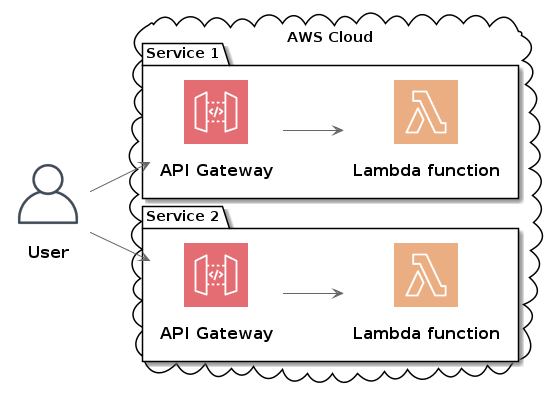
\includegraphics[width=7cm]{source/diagrams/multiple_api_gateway.png}
        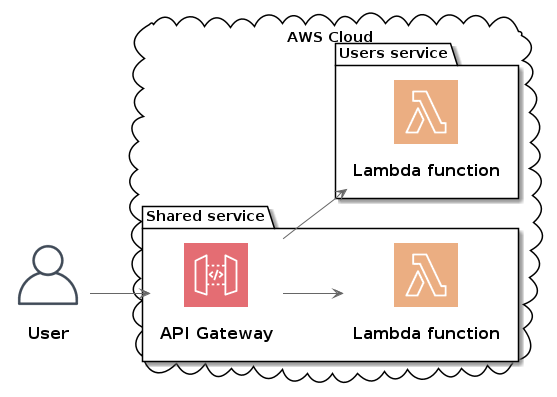
\includegraphics[width=7cm]{source/diagrams/single_api_gateway.png}
        \caption{Non shared (left) and shared (right) API Gateway on multiple services}
        \label{fig:api_gateway_multiple_services}.
    \end{figure}

    The \textit{JsonServices} class manages all operations regarding the Serverless
    services files, with the main ones being: offering CRUD methods for the various
    resources, such as: services; functions, with http or schedule events;
    serverless plugins; authorizer functions, associated to a single service or a
    shared authorizer.
    Each operation is reflected also on the \textit{offline} service.

    \subsubsection{Environment variables}
    \label{sec:env_vars}
    An important aspect when developing web applications is the handling of different
    deploying environments, as each one of them requires different configurations,
    mostly for sensitive information, such as database credentials.
    It has been decided to handle those information with different environment files,
    storing environment variables.
    When a project is created the framework generates 4 different environments: locale,
    test, staging and production. Each environment has an associated type and stage,
    with the first representing the purpose of that environment, and the latter the
    corresponding Serverless stage. Below are the available types:
    \begin{itemize}
        \item test: environments used only for testing, which can happen locally
            but also through CI platform.
        \item dev: environments used for local development.
        \item deploy: environments that can be deployed.
    \end{itemize}
    All information about the environments (name, type, stage) are stored in the
    configuration file \textit{config/envs.json} and are managed by the JsonEnvs
    class.

    Environment variables are stored in the format \textit{key=value} and variable
    expansions is supported, so the value of a key can be another variable, using
    the syntax shown on listing \ref{lst:env_key_syntax}.

    \bigskip
    \begin{code}[caption=Environment variable syntax, label={lst:env_key_syntax}]
key1=${otherKey}
key2=sample ${key1}
    \end{code}

    \noindent
    Each environment is then stored under the \mbox{\textit{envs/}} directory, in
    the form \mbox{\textit{.env.<name>}}, and the interaction with those files is
    handled by the \textit{EnvFile} class. The load and expansion operation is
    performed differently depending on the operation, local development or deploy.
    During local development it is the dev command that load the environment specified
    in input (\ref{sec:local_dev}). During deploy instead, the environment file
    is expanded and copied under the project root, in a file named .env, as this
    makes deploying from CI straightforward. Then at runtime the .env is automatically
    loaded by the LambdaHandler or ScheduleHandler functions.

    \subsubsection{Extensions}
    The framework has been designed from the beginning with the possibility of
    extending its functionalities using external packages.
    In order to achieve this, it has been defined an AddOnPackage class, containing
    the following lifecycle hooks:
    \begin{itemize}
        \item postInstall: executed after the addon package has been installed.
            Here it's possible to perform initialization operations.
        \item postEnvCreated: executed after a new environment has been created,
            so the addon can add its own environment variables if needed.
        \item beforeEndpoint: executed before the corresponding function of an
            endpoint. Here it's possible to perform resource initialization,
            for example opening a database connection.
        \item beforeSchedule: as for endpoints, it's executed before the
            corresponding function of a schedule.
    \end{itemize}
    In addition to this class Restlessness provides also more specific classes,
    for authentication and data access \ref{fig:rln_add_on_packages}.

    \begin{figure}
        \centering
        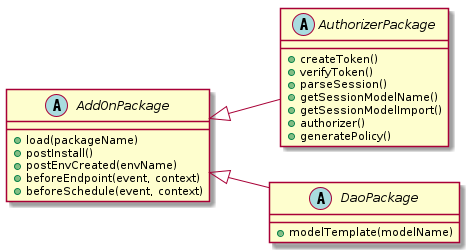
\includegraphics[width=10cm]{source/diagrams/rln_add_on_package.png}
        \caption{Add on packages structure}
        \label{fig:rln_add_on_packages}
    \end{figure}

    \subsubsection{Handlers}
    The Core package provides different functions and classes to simplify some
    operations and to provide additional functionalities on top of the Serverless
    framework.

    \paragraph{LambdaHandler} is a core function, reserved to be used for function
    associated with an http event. Its purpose is to parse the request payload and
    or query parameters, load the environment variables and execute the lifecycle
    hooks of the installed addons. After those operations the LambdaHandler executes
    the actual handler function associated for the endpoint.

    \paragraph{ScheduleHandler} behaves similarly to LambdaHandler, but it is
    reserved for functions with an associated schedule event, hence it is simpler.
    Its only tasks are to execute lifecycle hooks and the actual handler function.

    \paragraph{ResponseHandler} is a class providing static methods for generating
    response object for http endpoints. The response can be created using a JSON
    or a Buffer representation.

    \paragraph{TestHandler} is a class that simplify testing endpoints. Its main
    methods are: \textit{beforeAll}, \textit{afterAll} and \textit{invokeLambda}.
    The beforeAll function performs initialization operations, such as loading the
    correct environment variables and then the function invokeLambda executes the
    endpoint function providing automatically the event and context objects,
    simulating this way an http event. Then the afterAll function performs cleanup
    operations.
    The fact that serverless is based on function makes possible to use this simple
    testing structure, as it's not necessary for example to actually starts an http
    server to test the endpoints.

    \section{Cli}
    The Cli package provides a series of commands, listed here.

    \paragraph{new}
    Creates a new project in the current working directory, or on the specified
    input parameter.

    \paragraph{dev}
    \label{dev_command}
    The local development requires the presence of different processes, which are:
    the Api service and the Web Interface provided by Restlessness and also the
    project's process, to be able to test in real time the defined functions. The
    CLI handles those 3 processes through the dev command. In particular, both the
    project's process and Restlessness backend, are executed using the Serverless plugin
    \href{https://www.npmjs.com/package/serverless-offline}{serverless-offline},
    which allows simulating an api gateway, effectively creating a local http server.
    Instead for the frontend process it has been used the npm package
    \href{https://www.npmjs.com/package/serve}{serve}, through which is possible
    to create an http server that serves static files.
    Furthermore, the dev command takes care of executing those processes following the
    dependency order, which is: Restlessness backend, frontend and finally the
    project's process.
    Another task of the dev command is to implement inter process communication between
    itself and the backend process. This is necessary as when resources are created,
    for example endpoints or schedules, the corresponding files need to be compiled by
    typescript and also the serverless-offline plugin needs to be restarted for those
    resources to be available from the http server.
    The command receives the environment name in input, as it takes charge of loading
    the corresponding environment variables from the folder .envs, as explained on
    section \ref{sec:env_vars}. Among all environment variables, there is one, named
    \mbox{\textit{RLN\_PROJECT\_PATH}}, set by the \textit{dev} command, that indicates
    to the Backend process the path to the Restlessness project to manage.
    \begin{figure}
        \centering
        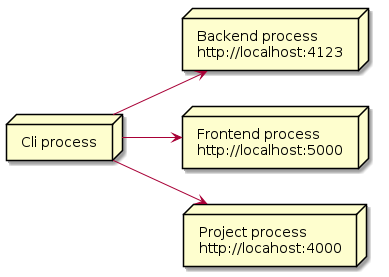
\includegraphics[width=7.5cm]{source/diagrams/rln_dev_processes.png}
        \caption{Processes generated by the dev command}
    \end{figure}

    \paragraph{create-env}
    Generates the \textit{.env} file, under project's root, corresponding to the
    environment name received as input.

    \paragraph{add-dao}
    Add an addon package of type Dao to the project, executing lifecycle hooks.

    \paragraph{add-auth}
    Add an addon package of type Auth to the project, executing lifecycle hooks.

    \paragraph{deploy}
    The Serverless Framework already provides a command for the deploy operation,
    as shown on \ref{sec:serverless_framework}, however with the micro services
    oriented structure suggested by Restlessness this operation is more elaborated,
    as it involves the deploy of more than one service, in a particular order.
    This is necessary because of the presence of the \textit{shared} resources
    service, so to successfully deploy a service that uses resources from the
    \textit{shared} one, it is necessary that those resources already exist.
    The correct deploy ordering is then \textit{shared} service first, followed
    by all the other services.
    It should be noted that the \textit{offline} service is not involved in the
    deploy process as it's used only for local development.
    To address this operations the Restlessness CLI provides a custom deploy
    command (listing \ref{lst:rln_command_deploy}).

    \bigskip
    \begin{code}[caption=Deploy command, label={lst:rln_command_deploy}, language=shell]
$ restlessness deploy
$ restlessness deploy --env production
$ restlessness deploy --env production users
    \end{code}

    It is possible to deploy the application on different environments, otherwise
    the command assume staging as the default environment.
    It is also possible to perform the deploy of just a single service, to keep
    the whole development, test and deploy process fast and easy, when making small
    changes, in accordance with the serverless paradigm.
    Since the deploy operation involves more than one service, it's important that
    the information among them are consistent, especially when deploying. This is
    why the deploy command, under the hood, takes care of performing this check,
    with a method from the \textit{JsonServices} class, named \textit{healthCheck}.
    In particular, it checks that the various services belong to the same serverless
    organization and organization, the same AWS deploy region, and that do not exist
    services with functions associated to the same path. The latter is due to the fact
    that the services use a shared api gateway.

    \paragraph{remove}
    Complementary command with respect to \textit{deploy}, it removes all services
    enforcing an opposite ordering doing so.

    \subsubsection{Backend}
    The Restlessness backend provides the endpoints used by the frontend to show,
    create, update and delete the framework resources described previously.
    It has been created with the Restlessness framework itself and it relies on
    the \mbox{\textit{@restlessness/core}} package to provide its functionalities.
    It is run locally using the
    \href{https://www.npmjs.com/package/serverless-offline}{serverless-offline}
    plugin, resulting in a lightweight Api Service.
    The Restlessness resources that the Api provides coincide with the resources
    already described, which are: Endpoints, Schedules, Authorizers, Daos, Envs,
    Models and Services.
    For each resource it has been created a corresponding Model, to map the information
    received from the core package into the format expected by the frontend, and
    vice versa. All Models inherit basic functionalities from a base class named
    \textit{BaseModel} (\ref{fig:base_model_class}), with utility methods for
    accessing data and the unimplemented methods \textit{toConfigEntry} and
    \textit{fromConfigEntry}, that perform map operations.
    Figure \ref{fig:backend_endpoint_flow} shows the flow for a request regarding
    the creation of an endpoint.

    \begin{figure}
        \centering
        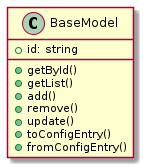
\includegraphics[width=3cm]{source/diagrams/rln_backend_base_model.png}
        \caption{BaseModel class}
        \label{fig:base_model_class}
    \end{figure}

    \begin{figure}
        \centering
        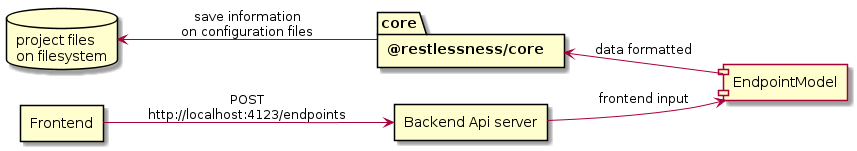
\includegraphics[width=\linewidth]{source/diagrams/rln_backend_endpoint_creation.png}
        \caption{Creation of an endpoint}
        \label{fig:backend_endpoint_flow}
    \end{figure}

    \subsubsection{Frontend}
    The Restlessness frontend provides a simple interface to interact with the
    framework. Once opened a dashboard provides some project's information and
    links to pages for each resource, where it is possible to view the current
    resources create, and modify them.
    Figure \ref{fig:frontend_site_map} shows the site map of the frontend.

    \begin{figure}
        \centering
        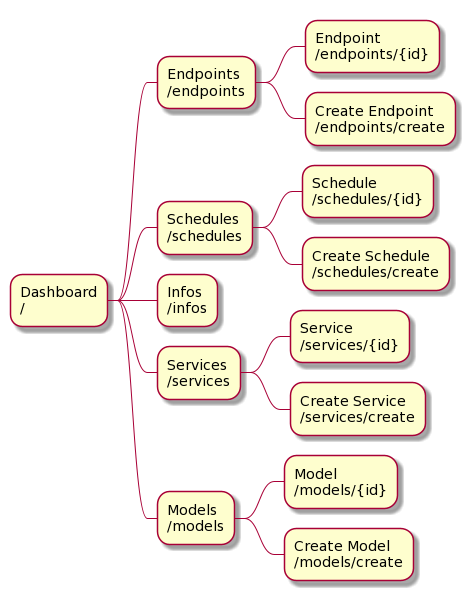
\includegraphics[width=8cm]{source/diagrams/frontend_site_map.png}
        \caption{Restlessness frontend site map}
        \label{fig:frontend_site_map}
    \end{figure}

    \section{Usage}
    \label{sec:rln_project_usage}

    The Restlessness CLI is available for installation on the npm platform. Once
    installed, the first step toward using the framework is the creation of a new
    project, and that is possible using the \textit{new} command, as shown
    on listing \ref{lst:rln_command_new}.

    \bigskip
    \begin{code}[caption=New command, label={lst:rln_command_new}, language=shell]
$ restlessness new rln_project
    \end{code}

    Once the command has finished, a new folder has been created, with a completely
    structured restlessness project, as can be see in figure
    \ref{fig:sample_rln_project_folder}.

    \begin{figure}
        \begin{minipage}{\linewidth}
            \dirtree{%
                .1 ./.
                .2 .restlessness.json.
                .2 configs/.
                .3 authorizers.json.
                .3 daos.json.
                .3 default-headers.json.
                .3 endpoints.json.
                .3 envs.json.
                .3 models.json.
                .3 schedules.json.
                .2 envs/.
                .3 .env.locale.
                .3 .env.production.
                .3 .env.staging.
                .3 .env.test.
                .2 serverless-services/.
                .3 offline.json.
                .3 shared.json.
                .2 src/.
                .3 exporter.ts.
                .3 schedulesExporter.ts.
            }
        \end{minipage}
        \caption{Sample Restlessness project structure}
        \label{fig:sample_rln_project_folder}
    \end{figure}

    The sample project shown in figure \ref{fig:sample_rln_project_folder} however,
    does not include all generated files, as some of them are not strictly part of
    the framework, but are required from other used tools, in particular:
    \begin{itemize}
        \item .eslintrc.json: configuration file of the linter
            \href{https://eslint.org/}{eslint}.
        \item .gitignore: it lists intentionally ignored files from the git tracking
            system.
        \item package.json: entry point of every npm project, it lists the project
            dependencies, as well as other project related information, such as
            the project name and version.
        \item package-lock.json: npm generated file, it contains a snapshot of the
            version of all dependencies, with the goal of obtaining reproducible
            builds.
        \item tsconfig.json: configuration file for the Typescript compiler.
    \end{itemize}

    The first noticeable difference with respect to a plain serverless project is the
    lack of a serverless.yml (or serverless.json) file under the root, instead it
    is present the \textit{serverless-services/} directory with the default services
    \textit{shared} and \textit{offline}.
    Other created files are: configuration files, under the \textit{config} folder,
    environment files, source code, under the src folder, and a .restlessness.json
    file, used to store project related information needed by the framework.

    \subsection{Local development}
    \label{sec:local_dev}

    The \textit{dev} command starts the processes as described on \ref{dev_command},
    producing the output shown on \ref{lst:rln_command_dev}.

    \bigskip
    \begin{code}[caption=Dev command, label={lst:rln_command_dev}, language=shell]
$ restlessness dev locale
$ RESTLESSNESS: Running on http://localhost:5000
$ rln-project: offline: Starting Offline: dev/us-east-1.
$ rln-project: offline: Offline listening on http://local...
$            * clean: rln-project-offline-dev-clean
$ rln-project:
$       POST | http://localhost:4000/dev/users
    \end{code}

    \subsection{Resource creation}
    The Web Interface looks like in the figure \ref{fig:rln_web_interface}, and
    provides some project details, such as serverless organization, application
    (section \ref{sec:serverless_framework}), and finally the aws data center
    region to which the project will be deployed.
    The main functionalities are then available through some shortcuts, that allow
    creating and consulting resources, such as endpoints, schedules, services and
    models.

    \begin{figure}
        \centering
        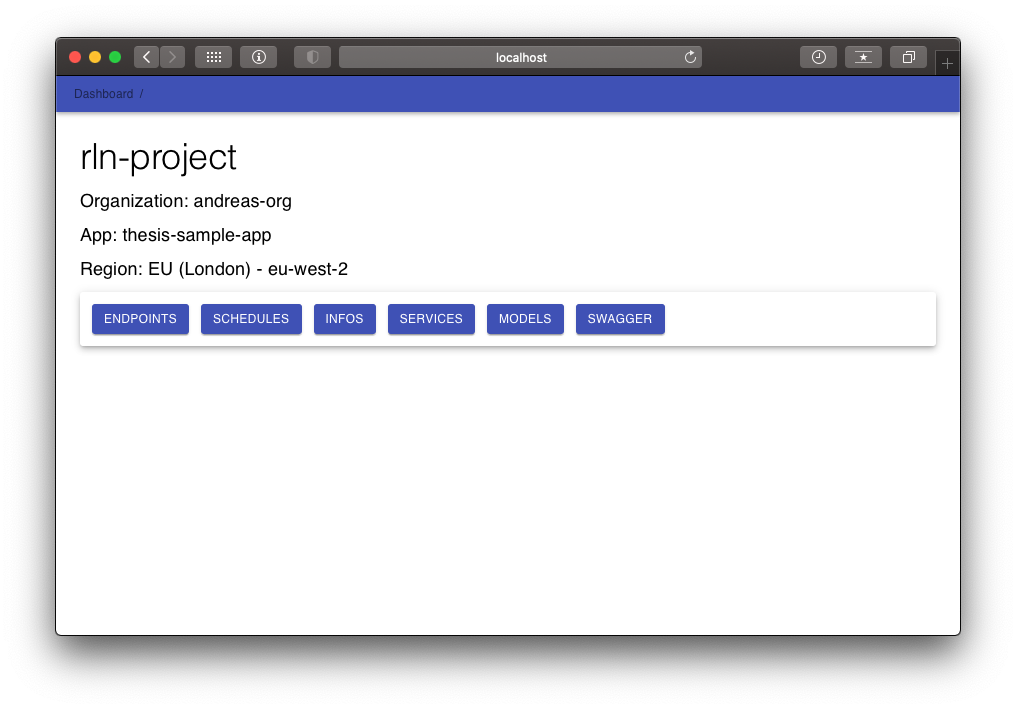
\includegraphics[width=\linewidth]{source/images/rln-web-interface.png}
        \caption{Restlessness Web Interface}
        \label{fig:rln_web_interface}
    \end{figure}

    Being Restlessness a framework for serverless services, the primary resource
    that can be defined are functions, and at the moment it is possible to define
    two type of functions, based on the event that triggers them. They are endpoints,
    and schedules.

    \subsubsection{Endpoints}
    \label{subsec:endpoints}
    It is possible to create an endpoint from the Web Interface, by specifying the
    following fields, as shown on figure \ref{fig:wi_create_endpoint}:
    \begin{itemize}
        \item Service: the service to which the function must be associated.
        \item Route: the path corresponding to the serverless function.
        \item Method: the http method.
        \item Warmup enabled: enable or disable the warmup plugin
            (\ref{subsec:cold_start})
        \item Daos: Associated Data Access Object addon.
        \item Authorizer: this optional field sets a further function, that
            perform the authorization operation, granting or denying access to
            the specified function.
    \end{itemize}

    \begin{figure}
        \centering
        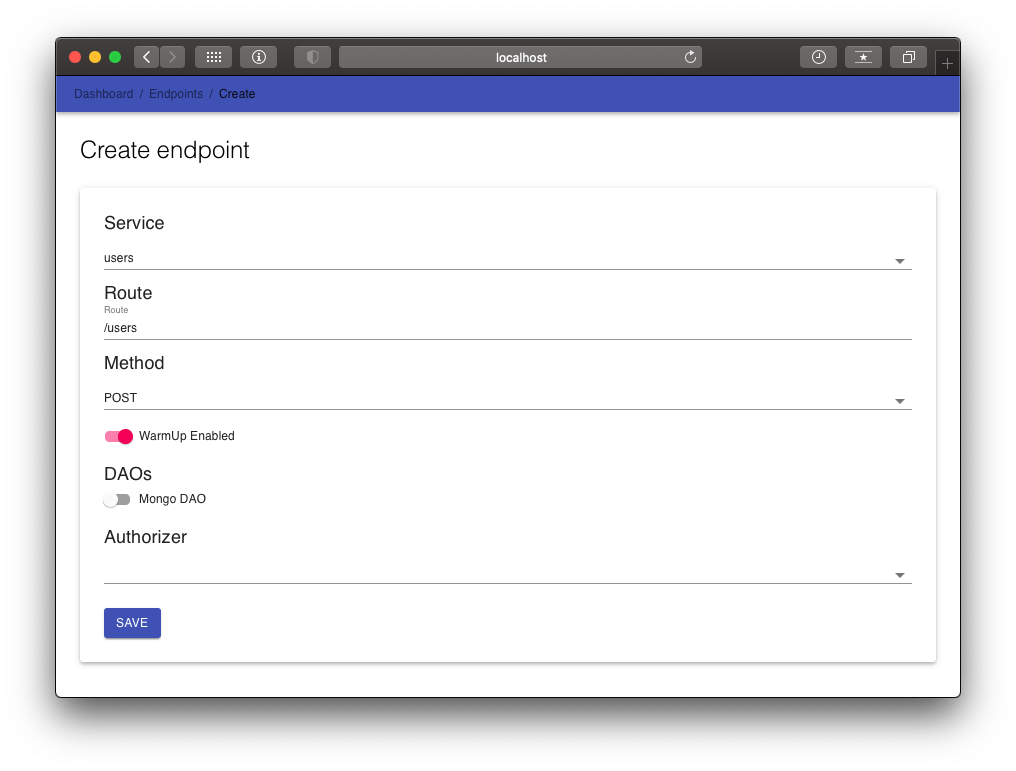
\includegraphics[width=\linewidth]{source/images/rln-wi-create-endpoint.png}
        \caption{Creation of and endpoint}
        \label{fig:wi_create_endpoint}
    \end{figure}

    During the endpoint creation, the framework takes care of saving the provided
    information on the configuration file \textit{config/endpoints.json}, and to
    create code template for the development of the corresponding function.
    As shown on figure \ref{fig:new_endpoint_folder_structure}, it has been created a
    folder under src/endpoints, using the notation http method plus normalized value
    of the http path.

    \begin{figure}
        \begin{minipage}{\linewidth}
            \dirtree{%
                .1 ./.
                .2 src/.
                .3 endpoints/.
                .4 post-users.
                .5 handler.ts.
                .5 index.ts.
                .5 index.test.ts.
                .5 interfaces.ts.
                .5 validations.ts.
                .3 exporter.ts.
                .3 schedulesExporter.ts.
            }
        \end{minipage}
        \caption{Structure of a new endpoint folder}
        \label{fig:new_endpoint_folder_structure}
    \end{figure}

    The developer can then code the function on the \textit{handler.ts} file, which
    already contains a template (listing \ref{lst:handler_ts}) and define the
    validation object in \textit{validations.ts} (listing \ref{lst:validations_ts}).
    It is also possible to exploit the Typescript functionalities, defining the various
    interface for the request, response and query parameters objects, all under the
    interfaces.ts file (listing \ref{lst:interfaces_ts}).
    The actual function entry point that will be executed once deployed is defined
    in the file \textit{index.ts} (listing \ref{lst:index_ts}). This function is
    created binding the function LambdaHandler input with the handler function and
    validation object.

    \clearpage

    \begin{code}[caption=handler.ts content, label={lst:handler_ts}]
export default async (req: Request) => {
  try {
    const {
        validationResult,
        payload,
    } = req;

    if (!validationResult.isValid) {
        return ResponseHandler.json({
            message: validationResult.message
        }, StatusCodes.BadRequest);
    }

    return ResponseHandler.json({});
  } catch (e) {
    console.error(e);
    return ResponseHandler.json(
        {}, StatusCodes.InternalServerError);
  }
};
    \end{code}

    \bigskip
    \begin{code}[caption=index.ts content, label={lst:index_ts}]
export default LambdaHandler
    .bind(this, handler, validations, 'postUsers');
    \end{code}

    \bigskip
    \begin{code}[caption=validations.ts content, label={lst:validations_ts}]
const queryStringParametersValidations =
  (): YupShapeByInterface<QueryStringParameters>  => ({});

const payloadValidations =
  (): YupShapeByInterface<Payload> => ({});

export default () => ({
  queryStringParameters: yup.object()
    .shape(queryStringParametersValidations()),
  payload: yup.object()
    .shape(payloadValidations()).noUnknown(),
});
    \end{code}

    \bigskip
    \begin{code}[caption=interfaces.ts content, label={lst:interfaces_ts}]
import { RequestI } from '@restlessness/core';
export interface QueryStringParameters {}
export interface Payload {}
export interface Request extends
    RequestI<QueryStringParameters, Payload, null> {};
    \end{code}

    \subsubsection{Schedules}
    \label{subsec:schedules}
    Schedules are serverless functions that are triggered by a programmed event.
    By creating a Schedule from the Web Interface the framework creates the necessary
    template files under \textit{src/schedules} as shown on
    \ref{fig:new_schedule_folder_structure}, and also saves the provided information
    under the \textit{config/schedules.json} file.

    \begin{figure}
        \begin{minipage}{\linewidth}
            \dirtree{%
                .1 ./.
                .2 src/.
                .3 schedules/.
                .4 clean/.
                .5 handler.ts.
                .5 index.ts.
            }
        \end{minipage}
        \caption{Structure of a schedule endpoint folder}
        \label{fig:new_schedule_folder_structure}
    \end{figure}

    The structure of the template files is similar to the one generated for endpoints,
    but simpler. The \textit{handler.ts} file contains the function that the developer
    has to code, while the \textit{index.ts} file is the entry point.
    The core function ScheduleHandler is used to wrap the handler function, the same
    way as happens for endpoints, with the purpose of executing the framework lifecycle
    hooks.

    \bigskip
    \begin{code}[caption=handler.ts content, label={lst:sched_handler_ts}]
export default async (event) => {};
    \end{code}

    \bigskip
    \begin{code}[caption=index.ts content, label={lst:sched_index_ts}]
import { ScheduleHandler } from '@restlessness/core';
import handler from './handler';
export default ScheduleHandler.bind(this, handler, 'clean');
    \end{code}

    \subsection{Test}
    A test template is also provided when creating a new endpoint, and it is based
    on the popular unit testing library \href{https://jestjs.io/}{jest}, in
    conjunction with the TestHandler class provided by Restlessness.

    \bigskip
    \begin{code}[caption=index.test.ts template, label={lst:endopints_test_ts}]
const postUsers = 'postUsers';

beforeAll(async done => {
  await TestHandler.beforeAll();
  done();
});

describe('postUsers API', () => {
  test('', async (done) => {
    const res = await TestHandler.invokeLambda(
        postUsers);
    // expect(res.statusCode).toBe(StatusCodes.OK);
    done();
  });
});

afterAll(async done => {
  await TestHandler.afterAll();
  done();
});
    \end{code}

\end{chapter}